\documentclass{tufte-handout}

%\geometry{showframe}% for debugging purposes -- displays the margins

\usepackage{amsmath}
\usepackage{amssymb}
\usepackage{amsthm}
\usepackage{thmtools}
\declaretheorem[numberwithin=section]
{theorem, definition}
\declaretheorem{lemma, proposition, corollary}[
style=plain,
numberwithin=theorem
]
% Set up the images/graphics package
\usepackage{graphicx}
\setkeys{Gin}{width=\linewidth,totalheight=\textheight,keepaspectratio}
\graphicspath{{graphics/}}

\title{MATH 454 Notes}
\author{Shan Gao}
\date{Fall 2023}

% The following package makes prettier tables.  We're all about the bling!
\usepackage{booktabs}

% The units package provides nice, non-stacked fractions and better spacing
% for units.
\usepackage{units}

% The fancyvrb package lets us customize the formatting of verbatim
% environments.  We use a slightly smaller font.
\usepackage{fancyvrb}
\fvset{fontsize=\normalsize}

% Small sections of multiple columns
\usepackage{multicol}

% Provides paragraphs of dummy text
\usepackage{lipsum}

% These commands are used to pretty-print LaTeX commands
\newcommand{\doccmd}[1]{\texttt{\textbackslash#1}}% command name -- adds backslash automatically
\newcommand{\docopt}[1]{\ensuremath{\langle}\textrm{\textit{#1}}\ensuremath{\rangle}}% optional command argument
\newcommand{\docarg}[1]{\textrm{\textit{#1}}}% (required) command argument
\newenvironment{docspec}{\begin{quote}\noindent}{\end{quote}}% command specification environment
\newcommand{\docenv}[1]{\textsf{#1}}% environment name
\newcommand{\docpkg}[1]{\texttt{#1}}% package name
\newcommand{\doccls}[1]{\texttt{#1}}% document class name
\newcommand{\docclsopt}[1]{\texttt{#1}}% document class option name


\begin{document}
	\maketitle
	\begin{abstract}
		These are my Analysis 3 notes, given in Fall 2023, by Professor Vétois 
	\end{abstract}
	\section{Measure theory}
\begin{definition}[Rectangle]
	For every rectangle $R = (a_1,b_1) \times (a_2,b_2) \times \cdot \times (a_d,b_d) \subseteq \mathbb{R}^d$ (can replace the open intervals with closed intervals), where $-\infty < a_i \leq b_i < \infty \quad \forall i$, we call the volume of $R$ $$\text{Vol}(R) = \prod_{i = 1}^d (b_i - a_i)$$. If $b_i - a_i = b_j - a_j \quad \forall i,j$, then we say that $R$ is a cube.
\end{definition}
\begin{definition}[exterior measure]
	For every set $A \subseteq \mathbb{R}^d$, we call exterior measure of $A$ and we denote $m_*(A)$ to be
	$$
	m_* (A) = \inf \{\sum_{k =1}^\infty \text{vol}(Q_k) \colon Q_k \text{ closed cubes such that } A \subseteq \bigcup_{k=1}^\infty Q_k\} 
	$$
	So we consider all possible coverings of $A$ by closed cubes and take the volume. A unbounded set doesn't mean that the measure is not finite. 
\end{definition}
In this course, convention is that we are using the extended real line, so $\infty$ and $-\infty$ are part of $\mathbb{R}$, the allowed operations are:
\begin{itemize}
	\item if $x$ is finite, then $x + \infty = \infty$
	\item $x -\infty = -\infty$
	\item any finite $x$ is $-\infty < x < +\infty$
	\item if $x$ is positive, then $x \cdot \infty = \infty$
	\item if $x$ is negative, then $-x \cdot \infty = -\infty$
	\item $\infty - \infty$ is undefined
	\item $0 \cdot \infty$ is sometimes defined to be $0$, otherwise undefined.
\end{itemize}
In the definition for exterior measures, we can replace the closed cubes by open cubes or rectangles in general. 
\begin{proposition}[exterior measure of a countable set]
	If $A \subseteq \mathbb{R}$ is countable, then the exterior measure $m_* (A) =0$
\end{proposition}
\begin{proof}
	Since $A$ is countable, there exists a sequence $(x_n \colon n \in \mathbb{N})$ in $\mathbb{R}^d$ such that $A = \{x_n \colon n \in \mathbb{N}\}$, since each of these points is a cube of volume $0$ following our definition, $A$ is a union of cubes of volume $0$, thus the exterior measure is $0$.
\end{proof}
\begin{proposition}[monotonicity of measure]
	If $A \subseteq B \subseteq \mathbb{R}$, then $m_* (A) \leq m_* (B)$
\end{proposition}
\begin{proof}
	Call $$ \tilde{A} = \{ \sum_{k=1}^\infty \text{Vol}(Q_k) \colon Q_k \text{ closed cubes such that } A \subseteq \bigcup_{k =1}^\infty (Q_k) \} \supseteq  \tilde{B} = \{ \sum_{k=1}^\infty \text{Vol}(Q_k) \colon Q_k \text{ closed cubes such that } B \subseteq \bigcup_{k =1}^\infty (Q_k) \} $$. As for why $\tilde{A} \supset \tilde{B}$ is because since $A$ is a smaller set there exists more ways of covering $A$ than $B$, and since the infimum of a bigger set is smaller, taking the infimum of $\tilde{A}$ and $\tilde{B}$, we get that $m_*(A) \leq m_* (B)$.  
\end{proof}
\begin{proposition}[Covering by mutually disjoint open cubes]
	Every open set $O \subseteq \mathbb{R}^d$ can be written as $O = \bigcup_{k = 1}^\infty \overline{Q}_k$ where $Q_k$ are mutually disjoint open cubes and $\tilde{Q}_k$ is the closure of $Q_k$. Furthermore, we can say that the exterior measure $$m_*(O) = \sum_{k=1}^\infty \text{Vol}(\overline{Q}_k)$$ 
	
\end{proposition}
\begin{proof}
	For each $k \in \mathbb{N}$, let $C_k$ be the set of all open cubes with vertices in the grid $2^{-k} \mathbb{Z}^d$, let $$C_k (O) = \{ Q \in C_k \colon \bar{Q} \subseteq O\}$$
	we call 
	$$ C_1(O) = \{Q \in C_1\colon \bar{Q} \subseteq O\}$$ and 
	$$ O_1 = \bigcup_{Q \in C_1(O)} \bar{Q}$$
	\begin{marginfigure}%
		
\includegraphics[width=\linewidth]{lec2ex1.png}
		\caption{example of grid}        
		\label{fig:ex1}
	\end{marginfigure}
	By induction, for each $k \geq 2$, we get that 
	$$
	C_k(O) = \{Q \in C_k \colon \bar{Q} \subseteq O \text{ and } \bar{Q} \subsetneq O_{k-1} \}
	$$
	and 
	$$O_{k-1} = \bigcup_{Q \in C_1(O) \cup \ldots \cup C_{k-1}(O)} \bar{Q}$$
	so we get that the $Q$ are disjoint by construction.
	With this construction we obtain 2 properties that we want $$\bigcup_{k=1}^\infty O_k \subseteq O = \bigcup_{k=1}^\infty \left(\bigcup_{Q \in C_k(O)} \bar{Q}\right)$$
	Their interiors will be completely disjoint, all the $C_k$'s are mutually disjoint. Now we need to prove the reverse inclusion. Intuitively, since the set is open we can take an open ball around any point and fit a cube inside it. Conversly, let $x \in O$, since for each $k \in \mathbb{N}$, letting $Q_{k,x}$ be an open cube such that $x$ belongs to $\overline{Q}_{k,x}$ since $O$ is open, and $2 ^{-k} \to 0$ as $k \to \infty$, we have that $\overline{Q}_{k,x} \subseteq O$ for large $k$. From our construction, we then obtain $\overline{Q}_{k,x} \subseteq O_k$ thus $$x \in \overline{Q}_{k,x} \subseteq \bigcup_{k=1}^\infty O_k$$, so we are done. By definition of $m_*(O)$, we have that $m_*(O) \leq \sum_{k=1}^\infty \text{Vol}(\overline{Q}_k)$ (the outer measure is the infimum of any such overing).\\
	Conversly, we need to consider another covering $(Q_j^\prime)_{j \in \mathbb{N}}$ be closed cubes such that $O \subseteq \bigcup_{j = 1}^\infty Q_j^\prime$. For every $j,k \in \mathbb{N}$,let $R_{j,k} = Q_j^\prime \cap \overline{Q}_k$ then $R_{j,k}$ is a rectangle. Since $O \subseteq \bigcup_{j = 1}^\infty Q_j ^\prime$, we obtain that for each $k \in \mathbb{N}$, $\overline{Q}_k \subseteq \bigcup_{j=1}^\prime R_{j,k}$ (Since all the $Q_j^\prime$ has to eventually cover $\overline{Q}_k$, it follows that $$\text{Vol}(\overline{Q}_k) \leq \sum_{j=1}^\infty \text{Vol}(R_{j,k})$$. On the other hand, since the cubes $Q_k$ are mutually disjoint, we obtain that for $j$ fixed, the rectangles $(R_{j,k})_{k \in \mathbb{N}}$ have also mutually disjoint interiors. Furthermore, these rectnalges $R_{j,k}$ are included in $Q_j^\prime$. 
	\begin{marginfigure}%
		
\includegraphics[width=\linewidth]{lec2ex2.png}
		\caption{Please don't hurt me}        
		\label{fig:hell}
	\end{marginfigure}

	It follows that 
	$$
		\sum_{k = 1}^\infty \text{Vol}(R_{j,k}) \leq \text{Vol}(Q_j^\prime)
	$$
	Therefore, we obtain that 
	$$
	\sum_{k=1}^\infty \text{Vol}(\overline{Q}_k) \leq \sum_{k=1}^\infty \left ( \sum_{j=1}^\infty \text{Vol}(R_{j,k}) \right) = \sum_{j=1}^\infty \left( \sum_{k=1}^\infty \text{Vol}(R_{j,k}) \right) \leq \sum_{j=1}^\infty \text{Vol}(Q_j ^\prime) 
	$$
	So any other covering has volume greater than our constructed covering, thus the infimum, taking the outer measure has $\sum_{k=1}^\infty \text{Vol}(\overline{Q}_k) \leq m_* (O)$, and we get the resulting equality
\end{proof}
\section{lecture 3}
First of all some corrections to the second lecture, if we have a sequence of rectangles $(R_k)_{k \in \mathbb{N}}$ that cover a rectangle $R$ then 
\begin{enumerate}
	\item[(i)] if $R \subseteq \bigcup_{k=1}^\infty R_k$ then $Vol(R) \leq \sum_{k=1}^\infty Vol(R_k)$
	\item[(ii)] if $\bigcup_{k=1}^\infty R_k \subseteq R$ and the rectangles are mutually disjoint then $\sum_{k=1}^\infty \leq Vol(R)$. 
\end{enumerate}
We prove these statements, if $Vol(R)=0$, then there is nothing to prove, otherwise, if $Vol(R) > 0$ , then let $R_\varepsilon$ be a compact (closed. since rectangles are already bounded) such that $R_\varepsilon \subseteq R$ such that
$$Vol(R_\varepsilon) > Vol(R) - \varepsilon$$
by shrinking the sides of the original rectangle $R$ (if needed). \\
Now let $R_{k, \varepsilon}$ be an \textbf{open} rectangle such that 
$$R_k \subseteq R_{k, \varepsilon}$$
and
$$Vol(R_{k, \varepsilon}) < Vol(R_k) + \varepsilon 2 ^k$$
\begin{marginfigure}%
	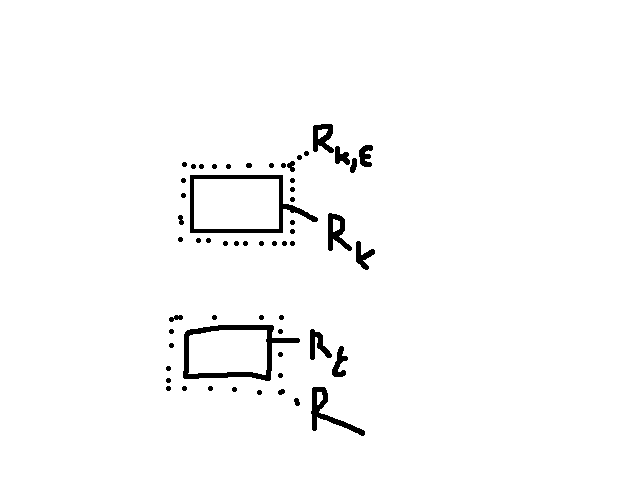
\includegraphics[width=\linewidth]{lec3fig1.png}
	\caption{don't do this to me}        
	\label{fig:lec3fig3}
\end{marginfigure}
we then get this nice inequality by taking the sum over the volumes for all $k$
$$ \sum_{k = 1}^\infty Vol(R_{k , \varepsilon}) < \sum_{k = 1}^\infty Vol(R_k) + \varepsilon \overbrace{\sum_{k=1}^\infty 2^k}^{\to 1}$$
We have that 
$$ R_\varepsilon \subseteq R \subseteq \bigcup_{k = 1}^\infty R_{k, \varepsilon} $$ . Note that $R_\varepsilon$ is compact, and $(R_{k , \varepsilon})_{k \in \mathbb{N}}$ is an open cover, so we can actually take a FINITE SUBCOVER (WOW!).Just in case you got lost in this vast, vast, vast, proof. Also, just in case you forgot, we're trying to prove (i) here, \textbf{remember} \footnote{or else you die trying to follow the rest}. Therefore, 
$$ \exists (R_{k_i, \varepsilon})_{1 \leq i \leq n}$$ 
such that $$R_\varepsilon \subseteq \bigcup_{i = 1}^n R_{k_i, \varepsilon}$$
Indeed, it covers $R_\varepsilon$ as well.
(I don't know what this mean I'm including this in here for future clarifications) By extending the sides of the rectangles of $R_\varepsilon$ and $R_{k_i, \varepsilon}$ we get that 
$$\sum_{i = 1}^n Vol(R_{k_i, \varepsilon}) - Vol(R) = \sum_{j = 1}^n Vol(R_j^\prime) $$ 
For some rectangles $(R_j^\prime)_{1 \leq j \leq n}$. 
It follows that 
$$Vol(R) - \varepsilon < Vol(R_\varepsilon) \leq \sum_{k=1}^n Vol(R_{k_i, \varepsilon}) \leq \sum_{k=1}^\infty Vol(R_{k, \varepsilon}) < \sum_{k = 1}^\infty Vol(R_k) + \varepsilon$$
Therefore we have,

$$Vol(R) - \varepsilon <  \sum_{k = 1}^\infty Vol(R_k) + \varepsilon $$, so we can conclude that a
$$Vol(R) \leq  \sum_{k = 1}^\infty Vol(R_k) $$
\subsection{outer measure (continued)}
For every rectangle $R$, we have that $m_* (R) = Vol(R)$
\begin{proof}
	Using the equivalent definition of $m_*(R)$ with rectangles (infimum of the volume of all possible coverings of $R$ with open/closed rectangles), since $R$ is one possible covering, then $m_*(R) \leq Vol(R)$. Conversly, consider coverings of that rectangle by rectangles. Let $(R_k)_{k \in \mathbb{N}}$ be rectangles such that 
	$$ R \subseteq \bigcup_{k = 1}^\infty R_k$$
	where 
	$$ Vol(R) \leq \sum_{k = 1}^\infty Vol(R_k)$$
	(see the proof of (i))
	And then we take the infimum on the right to get $Vol(R) \leq m_*(R)$ so the equality is shown	
\end{proof}
\begin{proposition}[measure of set infimum version ]
		For every set $A \subseteq \mathbb{R}^d$, $m_*(A) = \inf \{m_*(O) \colon O \text{ open set that contains } A\}$
	\end{proposition}
	\begin{proof}
		By Monotonicity since $A \subseteq O$, then $m_*(A) \leq m_*(O)$, hence  $m_*(A) \leq \inf \{m_*(O) \colon O\supset A\}$ 
		\begin{itemize}
			\item If $m_*(A) = \infty$ there is nothing more to prove
			\item If $m_*(A) < \infty$, we want to show that $m_*(A) \geq \inf\{m_*(O) \colon O \supset A\}$

		\end{itemize}
		But by using the equivalent definition of $m_*(A)$ with open cubes, there exists open cubes $(Q_k)_{k \in \mathbb{N}}$ such that 
		$$ A \subseteq \bigcup_{k = 1}^\infty Q_k \quad \text{ and } \quad \sum_{k = 1}^\infty Vol(Q_k) \leq m_*(A) + \varepsilon$$
		If $O_\varepsilon = \bigcup_{k=1}^\infty Q_k$, then $O_\varepsilon$ open in $\mathbb{R}^d$ and, since $A \subseteq O_\varepsilon$, and $m_*(O_\varepsilon) \leq \sum_{k=1}^\infty Vol(Q_k)$ by definition of outer measure of $O_\varepsilon$ since $(Q_k)_{k \in \mathbb{N}}$ is one possible covering of $O_\varepsilon$. It follows that 
		$$\inf\{m_*(O) \colon O \text{ open }, A \subseteq O\} \leq m_*(O_\varepsilon) \leq \sum_{k=1}^\infty Vol(Q_k) \leq m_*(A) + \varepsilon$$, thus letting $\varepsilon \to 0$, we get that 
		\[ \inf\{m_*(O) \colon O \text{ open }, A \subseteq O\} \leq m_*(A) + \varepsilon \]
	\end{proof}
	\begin{proposition}[Countable subadditivity]
		For every $(A_k)_{k \in \mathbb{N}}$ subsets of $\mathbb{R}^d$ 
		\[ Vol\left(\bigcup_{k =1}^\infty A_k \right) \leq \sum_{k=1}^\infty Vol(A_k) \implies m_*\left(\bigcup_{k=1}^\infty A_k \right) \leq \sum_{k=1}^\infty m_*(A_k) \]

	\end{proposition}
	\begin{proof}
		if $m_*(A_k) = \infty$ for some $k$, then there is nothing to prove. If $m_*(A)  < \infty$, then by definition, $\forall \varepsilon > 0$ there exists $(Q_{k,j,\varepsilon})_{j \in \mathbb{N}}$ closed cubes such that $A_k \subseteq \bigcup_{j=1}^\infty Q_{k,j,\varepsilon}$ and $\sum_{k=1}^\infty Vol(Q_{k,j,\varepsilon}) < m_*(A_k) + \varepsilon 2^{-k}$. Then 
		$$\bigcup_{k=1}^\infty A_k \subseteq \bigcup_{k=1}^\infty \bigcup_{j=1}^\infty Q_{k,j,\varepsilon}$$
		Which gives 
		$$m_*\left(\bigcup_{k=1}^\infty A_k\right) \leq \sum_{k \geq 1} \sum_{j \geq 1} Vol(Q_{k,j,\varepsilon}) \leq \sum_{k=1}^\infty m_*(A_k) + \varepsilon \sum_{k=1}^\infty 2^{-k}$$
		Letting $\varepsilon \to 0$, we then obtain what we watned $m_*(\bigcup_{k=1}^\infty A_k) \leq \sum_{k=1}^\infty m_*(A_k) $
	\end{proof}
	\begin{proposition}
		Let $A_1, A_2 \subseteq \mathbb{R}^d$ be such that $d(A_1,A_2) > 0$, then the sum of their outer measures
	\end{proposition}	

\end{document}
